
\section{Lab 2}
\subsection{Introduction}
In class we performed Gaussian Elimination on an image matrix to clarify the image; however, I still don't know how images are drawn using matrices and what the image matrix actually means. The goal of this lab is to create a gradient image using a matrix and scilab. This may sound excessively simple to some, but I really have no idea what I'm doing. I would really like to know how to generate matrix based images so I figured I could use this lab as a personal learning experience.

\subsection{Method}
There are several approaches I can take to solve this problem, and I will likely end up using all of these methods before I arrive at my final answer. One approach is to simply look up the answer from some source and attempt to replicate the method on my own. I feel like my personal learning experience will be most rewarding if I leave this solution as a last resort. Another approach is to make educated guesses and attempt to implement them until I arrive at a solution. While this is how I usually approach projects that interest me, I think I will attempt my next approach. The approach I will likely attempt first is to use the image data from class, make changes to the data, and note changes in the result. The last solution seems like the best approach since I will be starting with a working set of data. Before I get started with my chosen method I am going to attempt to make an educated guess as to how an image is generated using a matrix.

Using what I know about matrices and what I know about a two-dimensional image I am going to design my own method for displaying graphical matrices. I am assuming that horizontally arranged elements in a matrix will be referred to as rows and vertically arranged elements will be referred to as columns with a respective order of reference. A two-dimensional image will be a construct of points referred to individually as a point in a Cartesian-like coordinate system. Elements from the matrix will map directly to points on the image where the row and column of the matrix value will determine its location in the image and matrix elements value will determine the color that is displayed. I am going to use HTML5 and the Canvas element to model my design. I will build a Cartesian-like coordinate system with boxes to represent 1x1 image elements (pixels) and use a matrix or matrix-like data element (multidimensional arrays) to assign colors to the individual elements. I will attempt to create a word image similar to the one in the class exercise. Now that I have my best guess as to how I would design a matrix-based image I can move on to how matrix-images are implemented in SciLab.

For the SciLab portion of this Lab I will take the matrix generated as a result of the class exercise and change the values of the individual elements one-by-one until I can determine the effect of changing a value. Once I have discovered the result of changing values I will add an additional column of values and note how it changes the output. As a test I will proceed to add an additional row to the matrix and note any changes. If my guess is correct I should notice that changes to the values of the original matrix change colors on the rendered image, adding additional columns should extend the image on the Cartesian "x" axis, and adding additional rows should extend the image on the "y" axis. Once I have determined how matrix images are generated in Scilab I can procede to the final stage.

During the last stage I will create a gradient matrix-based image in Scilab. The image will fade from green to blue, left to right as clearly as possible. The image generated on my operating system may not me what you see with the same code, but I will include images of what I see on my screen. My operating system does some additional blurring so the gradient will likely look fantastic for me and pixellated for everyone not running Windows 8.

\subsection{Solution}
The first stage is implementation of my matrix-image design. To make life easy on myself I just used the standard RGB string as my matrix-element value.
\begin{lstlisting}[caption=Define Image Data]
var pixel = 20; //pixel size
var imagedata = [""];
imagedata[0] = ["#F00", "#FFF", "#F00", "#FFF", "#0F0", "#0F0", "#0F0"];
imagedata[1] = ["#F00", "#FFF", "#F00", "#FFF", "#FFF", "#0F0", "#FFF"];
imagedata[2] = ["#F00", "#F00", "#F00", "#FFF", "#FFF", "#0F0", "#FFF"];
imagedata[3] = ["#F00", "#FFF", "#F00", "#FFF", "#FFF", "#0F0", "#FFF"];
imagedata[4] = ["#F00", "#FFF", "#F00", "#FFF", "#0F0", "#0F0", "#0F0"];
var b = document.getElementById("image");
var board = b.getContext("2d");
board.canvas.height = imagedata.length * pixel;
board.canvas.width = imagedata[0].length * pixel;
for (i = 0; i < imagedata.length; i++) {
    for (j = 0; j < imagedata[i].length; j++) {
        board.fillStyle = imagedata[i][j];
        board.fillRect(j * pixel, i * pixel, pixel, pixel);
    }
}
\end{lstlisting}

\begin{figure}
\centering

\includegraphics[height=10em]{Lab2}
\caption{Output of imagedata}
\end{figure}

The next stage requires me to load the data from the in-class assignment and test my theoretical model. I'm not going to list the values out nor will I display the result here since I don't want to ruin the surprise for anyone who hasn't had the opportunity to figure it out. Loading the data into scilab and getting the result using our methods from lab I saved the result in x and plotted the image with Matplot(round(x)). The round is necessary for me because of my operating system. I changed the value of x(1,1) and the element in the first row and first column changed color while the others stayed the same. Using x(:,20) = 5; sets all of the values in column 20 to the color associated with 5 (red) and using x(6,:) = 7 adds a row to the bottom of the image that is the color associated with 7 (yellow). Your color associations may be different as 1 is black when I believe that it should be white (zero is also black). Since I am just messing with the values here I may as well determine which colors I will need to generate my gradient image in the next stage. After changing some of the values I find that green is associated with 3 and blue is associated with 2; however, there are no partial values in-between that I can build a gradient with.

\begin{figure}
\centering
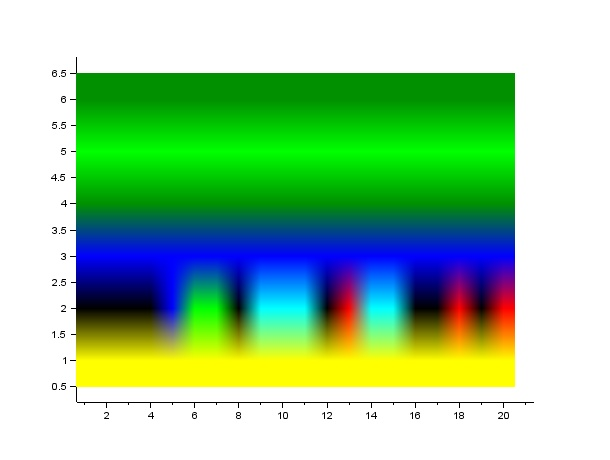
\includegraphics[height=20em]{lab2b}
\caption{in-class image after my tampering}
\end{figure}

\begin{figure}
\centering
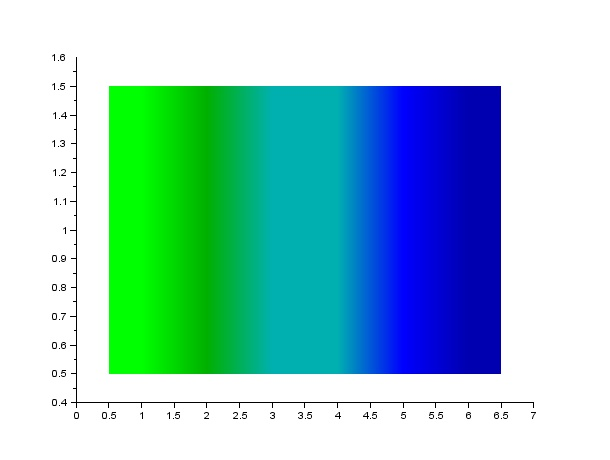
\includegraphics[height=20em]{ScilabGrad}
\caption{faux Scilab gradient}
\end{figure}

Since in-between values do not generate colors the way that I had imagined I am actually going to attempt to generate a faux gradient (figure 3). The Scilab only even looks close to a gradient because of my operating system. I'm sure that the color issue that I'm having is related to the operating system as well.

\begin{lstlisting}[caption=faux gradient]
clear
x(1,1) = 3;
x(1,2) = 14;
x(1,3) = 17;
x(1,4) = 17;
x(1,5) = 2;
x(1,6) = 10;
Matplot(x);
\end{lstlisting}

\subsection{Conclusion}
My conclusion is that Scilab is not completely supported on Windows 8 yet, and that my guess for matrix-image implementation was fairly accurate with (possibly) some differences in the the way that the color value is implemented. Basically Matrix-based images get the location of the element in the image based on the location in the matrix (row,column) and the value of the matrix element is associated with the color that is displayed.
